%%%%%%%%%%%%%%%%%%%%%%%%%%%%%%%%%%%%%%%%%%%%%%%%%%%%%%%%%%%%%%%%%%%%%%%%%%%%%%%
\section{Supplementary details for the spatial-discretization comparison}
\label{sec:supp-wp4}
%%%%%%%%%%%%%%%%%%%%%%%%%%%%%%%%%%%%%%%%%%%%%%%%%%%%%%%%%%%%%%%%%%%%%%%%%%%%%%%

\subsection{Stencil coefficients}

For offsets $r=-2,-1,0,1,2$, write
\[
 \mathcal A_i=\sum_r a_rE^r,\qquad
 \mathcal B_i=h^{-1}\sum_r b_rE^r,\qquad
 \mathcal C_i=h^{-3}\sum_r c_rE^r.
\]
The coefficient vectors are
\begin{align*}
 a^{\rm IT}&=(0,0,1,0,0),&
 b^{\rm IT}&=(0,-1/2,0,1/2,0),\\
 a^{\rm DF}&=(1,26,66,26,1)/120,&
 b^{\rm DF}&=(-1,-10,0,10,1)/24,\\
 a^{\rm P6}&=(1,56,126,56,1)/240,&
 b^{\rm P6}&=(-1,-10,0,10,1)/24,\\
 a^{\rm P8}&=(1,16,36,16,1)/70,&
 b^{\rm P8}&=(-5,-32,0,32,5)/84,
\end{align*}
and all four use
\[
 c=(-1/2,1,0,-1,1/2).
\]

\subsection{Profile and spectral verification}

Tables `nyquist_profile_summary.csv` and `spatial_floquet_summary.csv` in the
reproducibility archive give iteration counts, integral identities, fixed-point
residuals, eigenpair residuals, and both midpoint and GL4 spectra.  Pad\'e-6
GL4 refinement from $\kappa=5$ to $20$ changes the leading spectral radius
from $1.1558858$ to $1.1559821$.

\subsection{Natural simulations}

Figures~\ref{fig:supp-wp4-it}--\ref{fig:supp-wp4-p8} show moving-edge-frame
spacetime diagrams of the absolute Nyquist high-pass component.  The Pad\'e-6
run was continued to $T=30$; the automated profile search found no candidate
with own-family relative residual below $0.02$, with best value $0.528$.
This is reported as a finite-window observation, not as absence of nonlinear
shedding for all phases or times.

\begin{figure}[t]
 \centering
 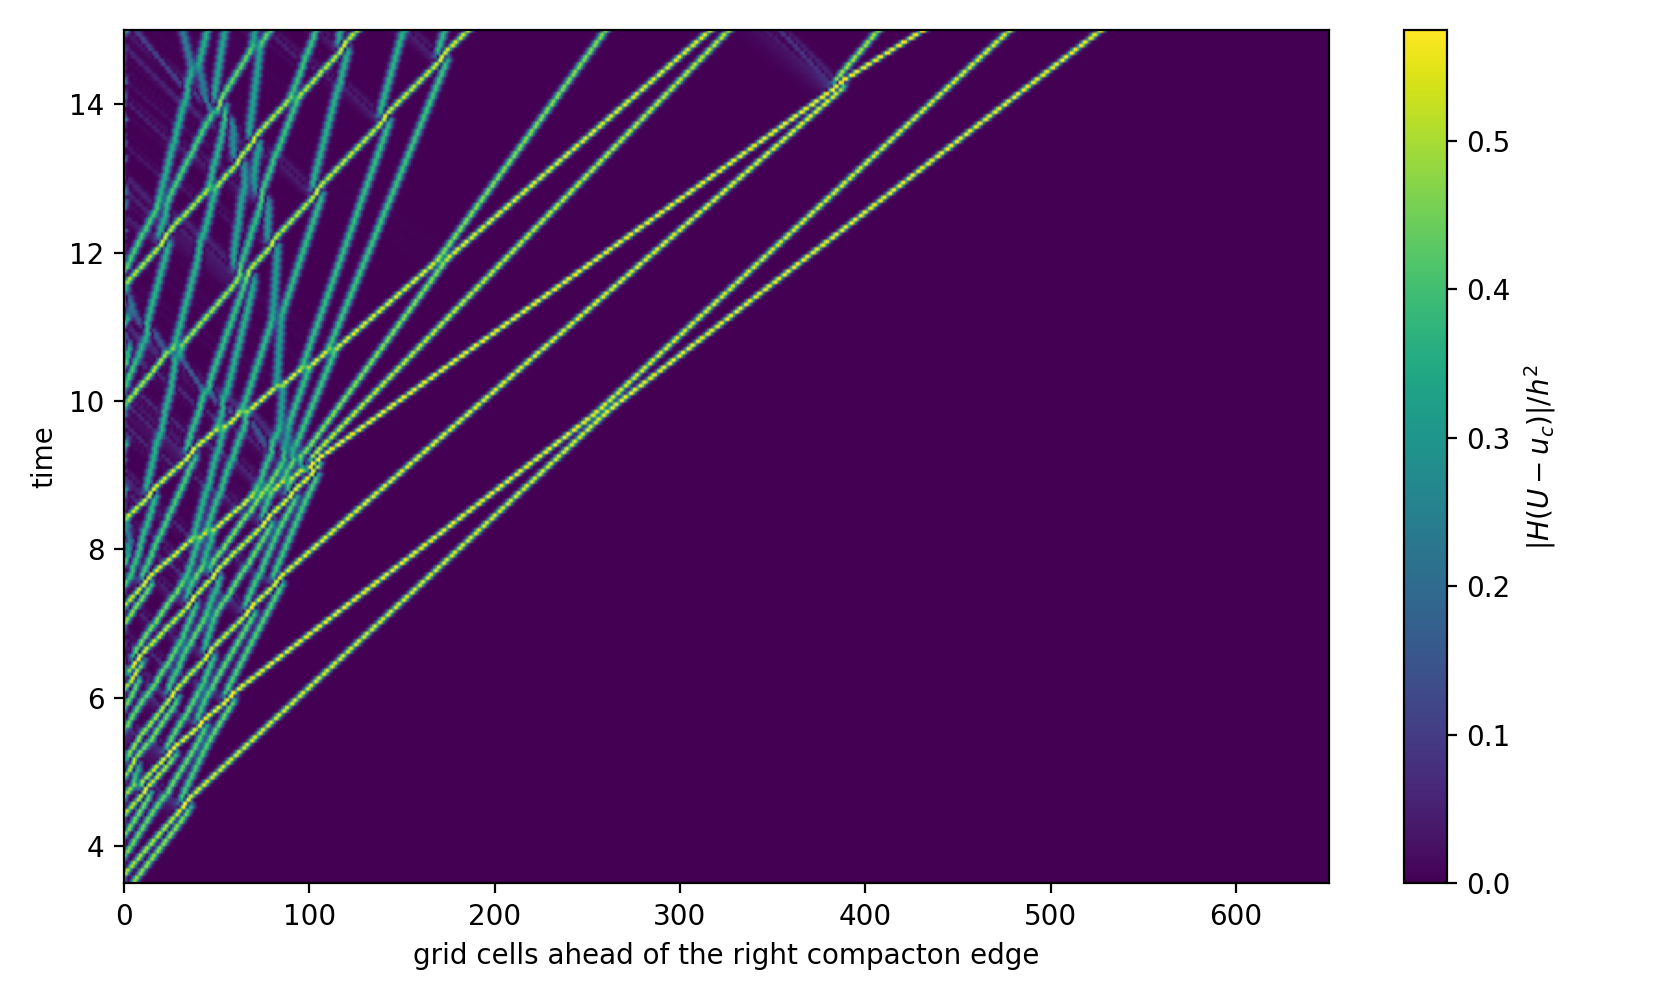
\includegraphics[width=0.88\textwidth]{wp4_spacetime_ismail.png}
 \caption{Ismail--Taha forward Nyquist field in the moving edge frame.}
 \label{fig:supp-wp4-it}
\end{figure}
\begin{figure}[t]
 \centering
 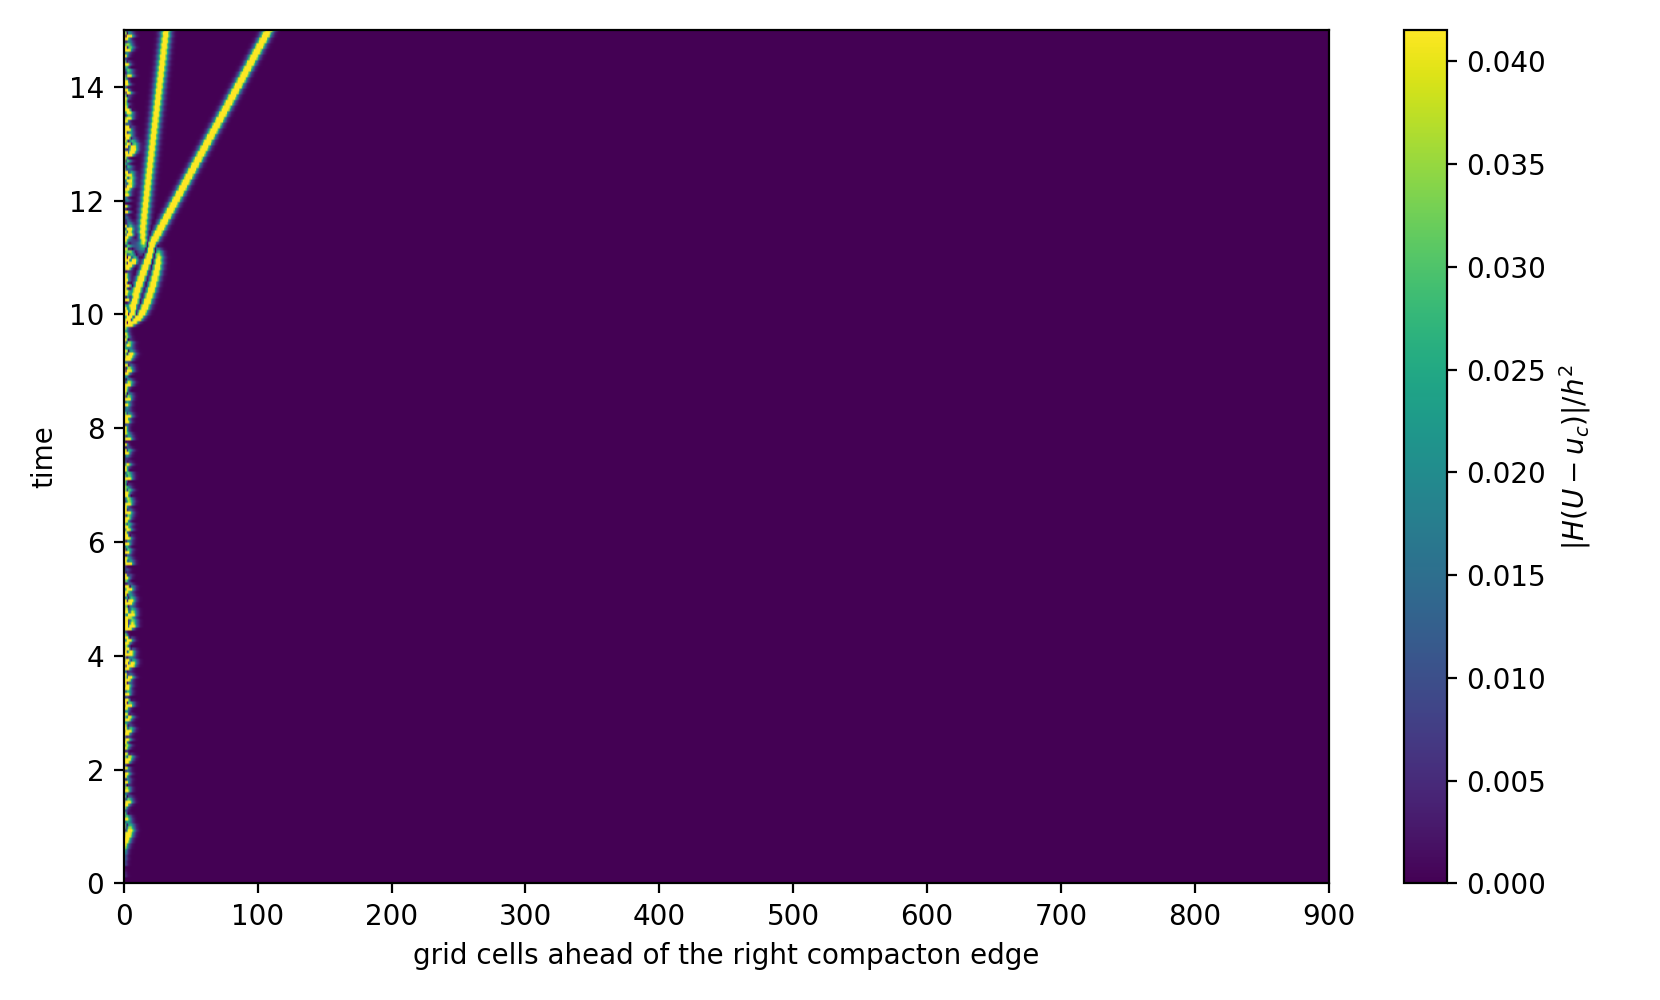
\includegraphics[width=0.88\textwidth]{wp4_spacetime_defrutos.png}
 \caption{de Frutos forward Nyquist field in the moving edge frame.}
 \label{fig:supp-wp4-df}
\end{figure}
\begin{figure}[t]
 \centering
 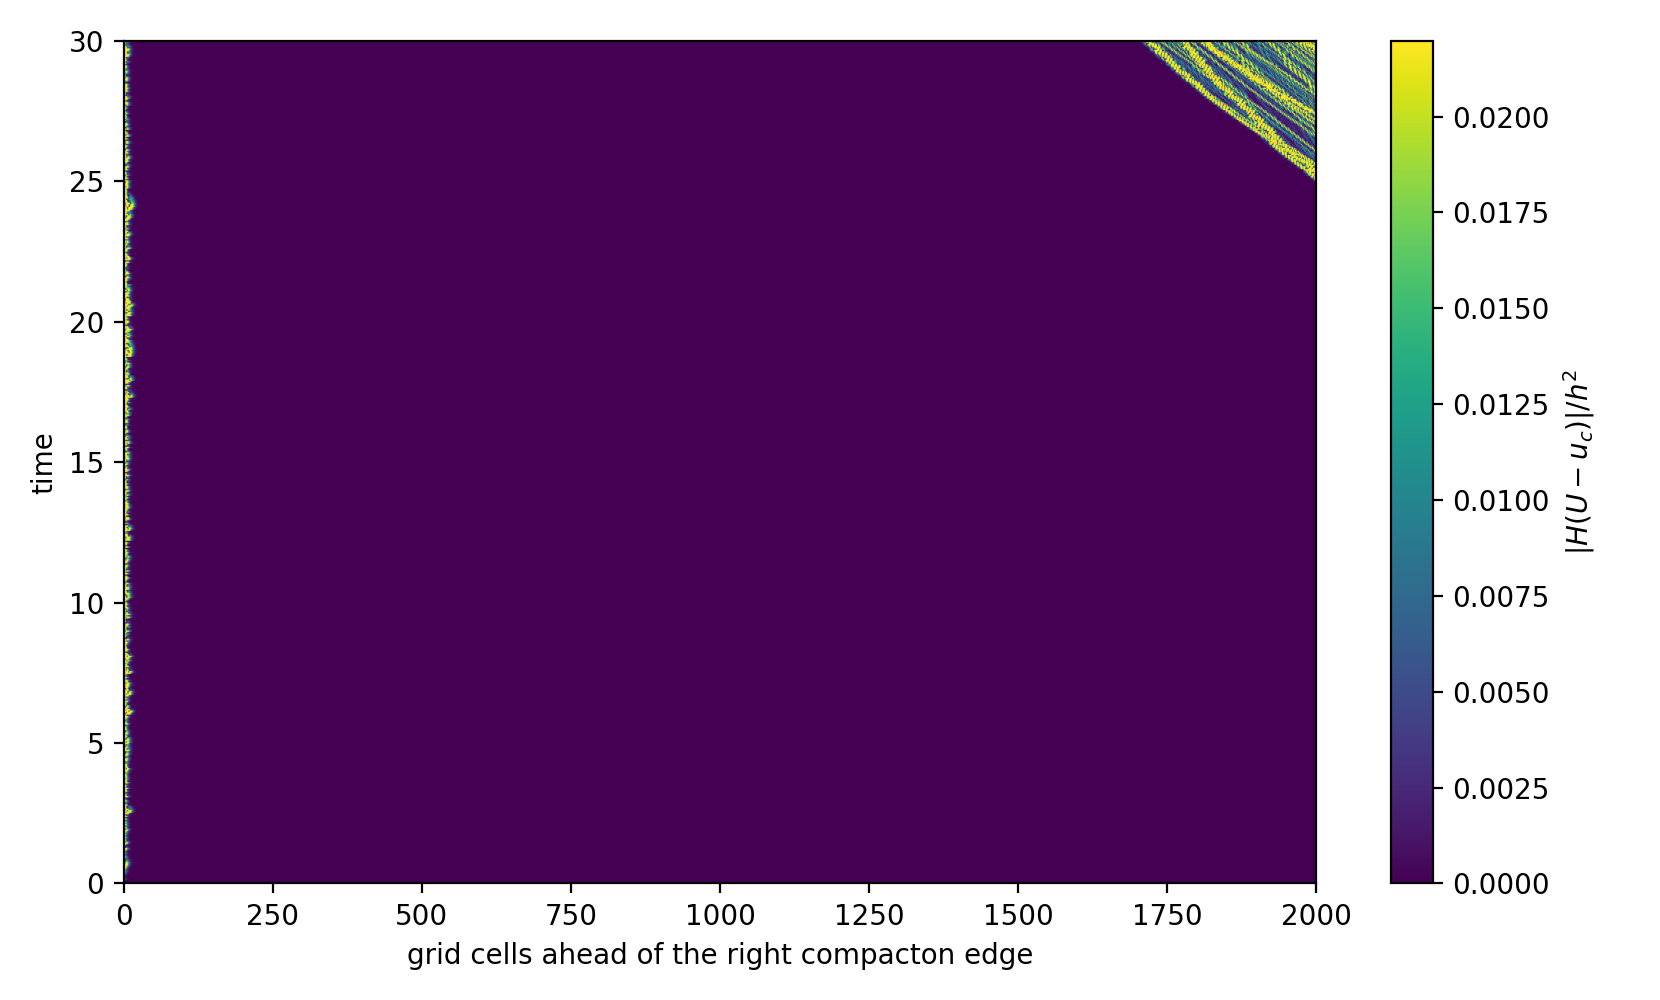
\includegraphics[width=0.88\textwidth]{wp4_spacetime_pade6.png}
 \caption{Pad\'e-6 forward Nyquist field in the moving edge frame.}
 \label{fig:supp-wp4-p6}
\end{figure}
\begin{figure}[t]
 \centering
 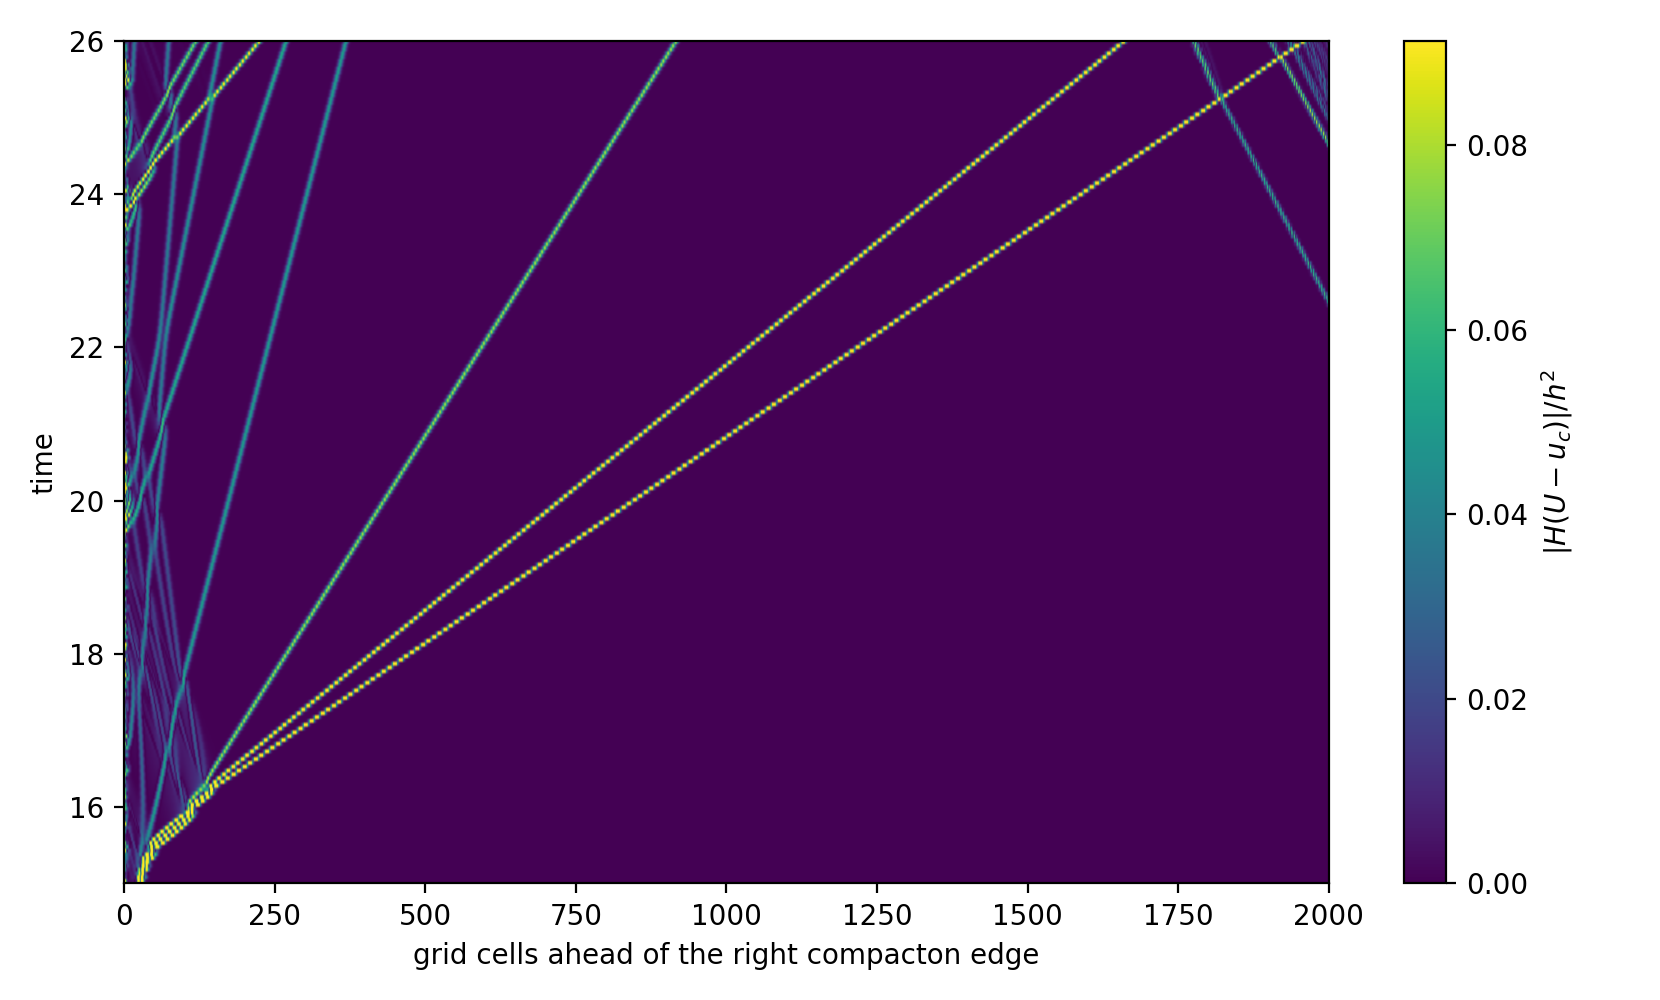
\includegraphics[width=0.88\textwidth]{wp4_spacetime_pade8.png}
 \caption{Pad\'e-8 forward Nyquist field in the moving edge frame.}
 \label{fig:supp-wp4-p8}
\end{figure}

\subsection{Independent and cross-family validation}

The complete natural and prepared-wave tracks are in
`natural_packet_snapshot_fits.csv` and
`natural_vs_prepared_wave_validation.csv`.  Cross-fitting the two
representative natural packets with all four profiles is reported in
`cross_profile_specificity.csv` and summarized in
Fig.~\ref{fig:supp-wp4-cross}.

\begin{figure}[t]
 \centering
 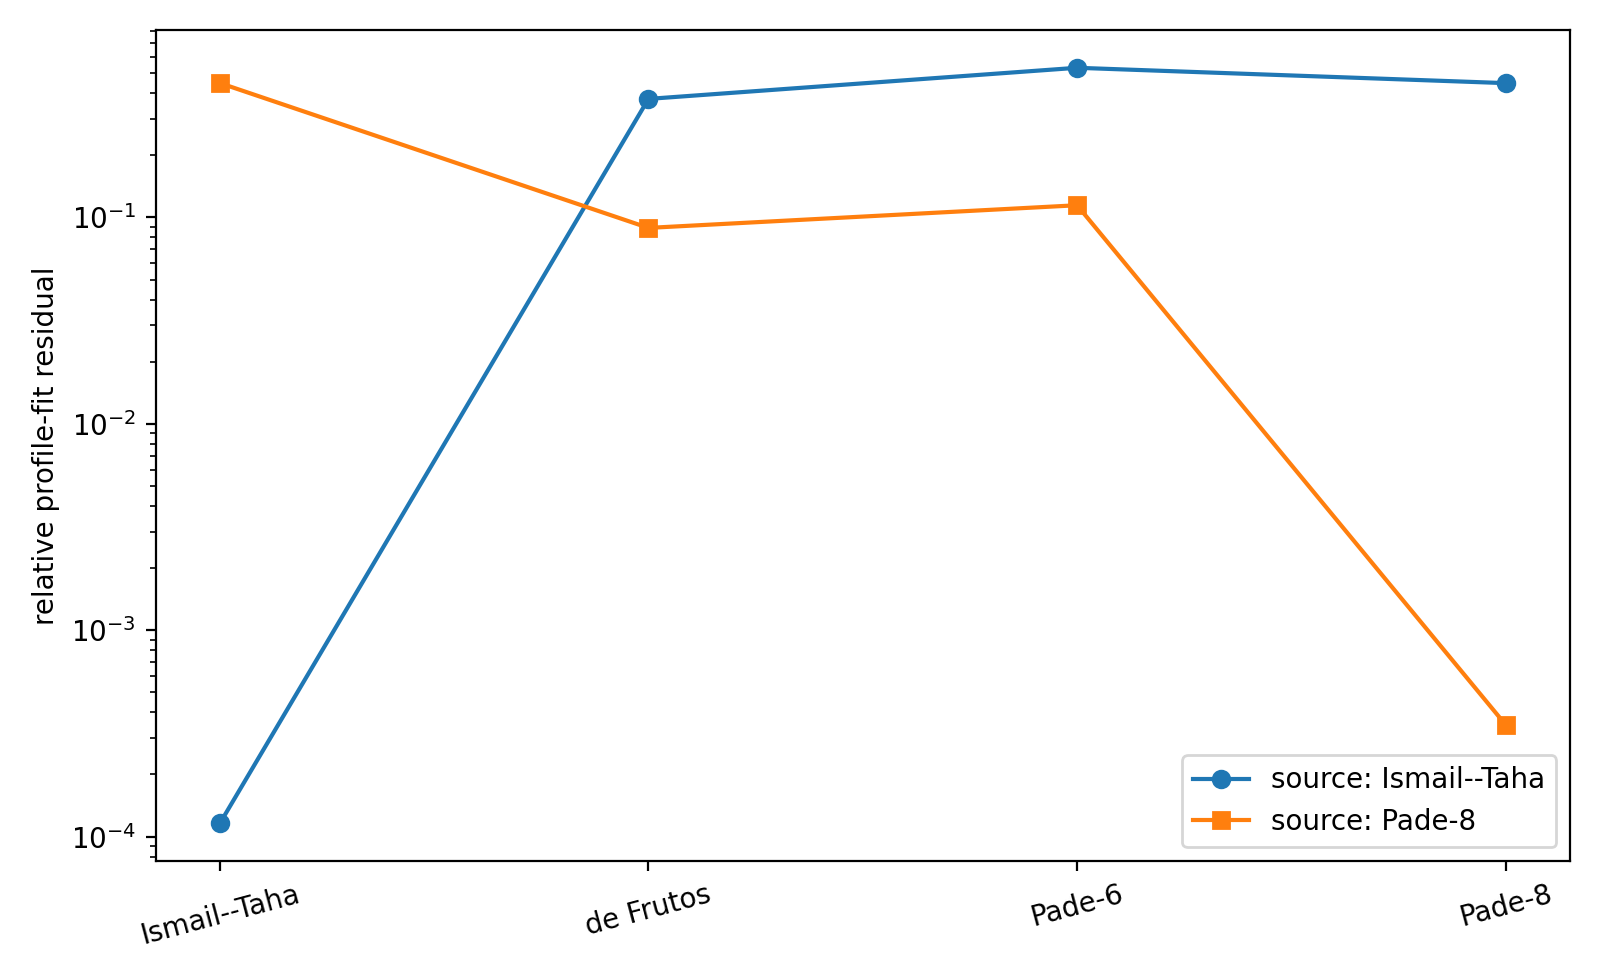
\includegraphics[width=0.72\textwidth]{wp4_cross_profile_specificity.png}
 \caption{Relative residual obtained when clean natural packets are fitted
 with the four stencil-specific profile families.}
 \label{fig:supp-wp4-cross}
\end{figure}
